\subsection{Bounded Sets and Metric Sequences}

\begin{definition} \label{def:bounded-and-perfect-metric-sets} \hlt{Bounded and Perfect Metric Sets}\\
Let $(X,d)$ be a metric space and let $E\subseteq X$.
\begin{enumerate}[label=(\roman*)]
\setlength{\itemsep}{0pt}
\item The set $E$ is \hlt{bounded} iff $(\exists q\in X)(\exists M>0)\,E\subseteq B_M(q)$.
\item The set $E$ is \hlt{perfect} iff $E$ is closed and $(\forall p\in E)\,p\in E^{\operatorname{acc}}$.
\end{enumerate}
\end{definition}

\begin{definition} \label{def:sequence-convergence-metric} \hlt{Metric Convergence}\\
Let $(p_n)$ be a sequence in a metric space $(X,d)$. It \hlt{converges} to $p\in X$ iff $(\forall\varepsilon>0)(\exists N\in\N)(\forall n\geq N)\,d(p_n,p)<\varepsilon$.\\
Write $p_n\to p$ or $\lim\limits_{n\to\infty}p_n=p$. The sequence \hlt{diverges} iff $(\nexists p\in X)\,p_n\to p$.
\end{definition}

\begin{definition} \label{def:sequence-range-and-boundedness} \hlt{Metric Sequence Terminology}\\
Let $p:\N\to X$, $n\mapsto p_n$, be a sequence in a metric space $(X,d)$.
\begin{enumerate}[label=(\roman*)]
\setlength{\itemsep}{0pt}
\item The \hlt{range} of $(p_n)$ is $\operatorname{ran}(p_n)\defeq\{p_n:n\in\N\}$.
\item The sequence $(p_n)$ is \hlt{bounded} iff $\operatorname{ran}(p_n)$ is bounded.
\item If $\sigma:\N\to\N$ satisfies $(\forall k\in\N)\,\sigma(k+1)>\sigma(k)$, then $(p_{\sigma(k)})_{k\in\N}$ is a \hlt{subsequence} of $(p_n)$.
\item A point $q\in X$ is a \hlt{subsequential limit} of $(p_n)$ iff $(\exists\,\sigma:\N\to\N)\,[(\forall k\in\N)\,\sigma(k+1)>\sigma(k)\land p_{\sigma(k)}\to q]$.
\end{enumerate}
\end{definition}

\begin{definition} \label{def:eventually-and-frequently-in-a-set} \hlt{Eventual and Frequent Membership}\\
Let $X$ be a set, let $(p_n)$ be a sequence in $X$, and let $E\subseteq X$.
\begin{enumerate}[label=(\roman*)]
\setlength{\itemsep}{0pt}
\item The sequence $(p_n)$ is \hlt{eventually in $E$} iff $(\exists N\in\N)(\forall n\geq N)\,p_n\in E$.
\item The sequence $(p_n)$ is \hlt{frequently in $E$} iff $(\forall N\in\N)(\exists n\geq N)\,p_n\in E$.
\end{enumerate}
\end{definition}

\begin{perspective} \label{per:metric-sequences-as-topological-tests} \hlt{Sequences as Metric Tests}\\
Definitions \ref{def:sequence-convergence-metric} and \ref{def:eventually-and-frequently-in-a-set} separate tail control from arbitrarily late recurrence.\\
In metric spaces, sequences convert local ball conditions into countable tests; this viewpoint does not replace the ball definitions.
\end{perspective}

\begin{theorem} \label{thm:metric-sequence-basic-properties} \hlt{Basic Properties of Metric Convergence}\\
Let $(p_n)$ be a sequence in a metric space $X$, let $E\subseteq X$, and let $p,p'\in X$.
\begin{enumerate}[label=(\roman*)]
\setlength{\itemsep}{0pt}
\item $p_n\to p\Longleftrightarrow (\forall r>0)(\exists N\in\N)(\forall n\geq N)\,p_n\in B_r(p)$.
\item $p_n\to p\land p_n\to p'\Longrightarrow p=p'$.
\item $p\in E^{\operatorname{acc}}\Longrightarrow(\exists q:\N\to E\setminus\{p\})\,q_n\to p$.
\end{enumerate}
\begin{proof}
\begin{enumerate}[label=(\roman*)]
\setlength{\itemsep}{0pt}
\item[$(i)$] ($\Rightarrow$) Let $r>0$. Some $N\in\N$ satisfies $(\forall n\geq N)\,p_n\in B_r(p)$ by Definition \ref{def:sequence-convergence-metric} with $\varepsilon=r$.
\item[$(i)$] ($\Leftarrow$) Let $\varepsilon>0$. Choose $N\in\N$ with $(\forall n\geq N)\,d(p_n,p)<\varepsilon$ by the ball condition at $r=\varepsilon$. Then $p_n\to p$ by Definition \ref{def:sequence-convergence-metric}.
\item[$(ii)$] Suppose $p_n\to p$, $p_n\to p'$, and $p\neq p'$. Set $\delta\defeq d(p,p')>0$.\\
Choose $N,N'\in\N$ with $(\forall n\geq N)\,d(p_n,p)<\frac{\delta}{2}$ and $(\forall n\geq N')\,d(p_n,p')<\frac{\delta}{2}$.\\
For $n\geq\max\{N,N'\}$, $\delta\leq d(p,p_n)+d(p_n,p')<\delta$ by the triangle inequality, a contradiction.
\item[$(iii)$] Suppose $p\in E^{\operatorname{acc}}$. Choose $(q_n)$ with $(\forall n\in\N)\,q_n\in(E\setminus\{p\})\cap B_{\frac{1}{n}}(p)$.\\
Given $\varepsilon>0$, choose $N\in\N$, $N\varepsilon>1$ by Theorem \ref{thm:archimedean-and-rational-density}(i). Then $(\forall n\geq N)\,d(q_n,p)<\frac{1}{n}\leq\frac{1}{N}<\varepsilon$, so $q_n\to p$ by Definition \ref{def:sequence-convergence-metric}.
\end{enumerate}
\hlt{Structural Commentary}: Ball membership restates the metric bound; shrinking punctured balls construct the approximating sequence.\\
\hlt{Key Insight}: The triangle inequality forbids two distinct limits.
\end{proof}
\end{theorem}

\begin{corollary} \label{cor:metric-convergent-subsequences} \hlt{Subsequences Preserve Metric Limits}\\
Let $(p_{n_k})$ be a subsequence of $(p_n)$ in a metric space. If $p_n\to p$, then $p_{n_k}\to p$.
\begin{proof}
The bound $(\forall k\in\N)\,n_k\geq k$ holds by induction from strict increase. Given $\varepsilon>0$, choose $N\in\N$ with $(\forall n\geq N)\,d(p_n,p)<\varepsilon$.\\
Then $(\forall k\geq N)\,n_k\geq k\geq N$, so $d(p_{n_k},p)<\varepsilon$ and $p_{n_k}\to p$ by Definition \ref{def:sequence-convergence-metric}.\\
\hlt{Structural Commentary}: Strictly increasing indices place every subsequence tail inside the corresponding original tail.\\
\hlt{Key Insight}: Deleting terms preserves every eventual metric bound.
\end{proof}
\end{corollary}

\begin{proposition} \label{prop:sequence-limit-points-subsequential-limits} \hlt{Subsequential Limit Criterion}\\
Let $(p_n)$ be a sequence in a metric space $X$ and let $p\in X$. The following are equivalent:
\begin{enumerate}[label=(\roman*)]
\setlength{\itemsep}{0pt}
\item $(\forall r>0)(\forall N\in\N)(\exists n\geq N)\,p_n\in B_r(p)$.
\item $(\exists\,\sigma:\N\to\N)\,[(\forall k\in\N)\,\sigma(k+1)>\sigma(k)\land p_{\sigma(k)}\to p]$.
\end{enumerate}
\begin{proof}
\begin{enumerate}[label=(\roman*)]
\setlength{\itemsep}{0pt}
\item[$(i)$] $\Rightarrow (ii)$ Set $n_0\defeq0$. Given $n_{k-1}$, let $I_k\defeq\{n\geq n_{k-1}+1:p_n\in B_{\frac{1}{k}}(p)\}$.\\
The set $I_k$ is nonempty by (i); define $n_k\defeq\min I_k$ by well-ordering. Thus $n_k>n_{k-1}$ and $d(p_{n_k},p)<\frac{1}{k}$.\\
Given $\varepsilon>0$, choose $K\in\N$, $K\varepsilon>1$ by Theorem \ref{thm:archimedean-and-rational-density}(i). Then $(\forall k\geq K)\,d(p_{n_k},p)<\frac{1}{k}\leq\frac{1}{K}<\varepsilon$, so $p_{n_k}\to p$ by Definition \ref{def:sequence-convergence-metric}.
\item[$(ii)$] $\Rightarrow (i)$ Write $n_k\defeq\sigma(k)$. The bound $(\forall k\in\N)\,n_k\geq k$ holds by induction from strict increase.\\
Given $r>0$ and $N\in\N$, choose $K\in\N$ with $(\forall k\geq K)\,d(p_{n_k},p)<r$. For $k\geq\max\{K,N\}$, $n_k\geq k\geq N$ and $p_{n_k}\in B_r(p)$.
\end{enumerate}
\hlt{Structural Commentary}: Repeated late ball visits support increasing indices with errors bounded by $k^{-1}$.\\
\hlt{Key Insight}: Increasing indices turn recurrence at every scale into subsequential convergence.
\end{proof}
\end{proposition}

\begin{proposition} \label{prop:discrete-metric-convergence-eventually-constant} \hlt{Discrete-Metric Convergence}\\
Let $X$ carry the discrete metric, let $(p_n)$ be a sequence in $X$, and let $p\in X$. Then $p_n\to p\Longleftrightarrow(\exists N\in\N)(\forall n\geq N)\,p_n=p$.
\begin{proof}
\begin{enumerate}[label=\roman*.]
\setlength{\itemsep}{0pt}
\item[$(\Rightarrow)$] Suppose $p_n\to p$. With $\varepsilon=\frac{1}{2}$, choose $N\in\N$ such that $(\forall n\geq N)\,d(p_n,p)<\frac{1}{2}$.\\
Since $d(X\times X)\subseteq\{0,1\}$, $(\forall n\geq N)\,d(p_n,p)=0$, so $(\forall n\geq N)\,p_n=p$.
\item[$(\Leftarrow)$] Choose $N\in\N$ with $(\forall n\geq N)\,p_n=p$. Then $(\forall\varepsilon>0)(\forall n\geq N)\,d(p_n,p)=0<\varepsilon$, so $p_n\to p$ by Definition \ref{def:sequence-convergence-metric}.
\end{enumerate}
\hlt{Structural Commentary}: The threshold $\frac{1}{2}$ converts the convergence tail into a zero-distance tail.\\
\hlt{Key Insight}: In the discrete metric, $d(x,y)<1\Longleftrightarrow x=y$.
\end{proof}
\end{proposition}

\begin{definition} \label{def:equivalent-metrics} \hlt{Equivalent Metrics}\\
Let $X$ be a set and let $\rho,\sigma:X\times X\to[0,\infty)$ be metrics.\\
They are \hlt{equivalent}, written $\rho\sim\sigma$, iff $(\exists c_1,c_2>0)(\forall x,y\in X)\,c_1\sigma(x,y)\leq\rho(x,y)\leq c_2\sigma(x,y)$.
\end{definition}

\begin{proposition} \label{prop:equivalent-metrics-preserve-tests} \hlt{Equivalent Metrics Preserve Topological Tests}\\
Let $X$ be a set, $\rho\sim\sigma$ be metrics on $X$, $\tau_\rho,\tau_\sigma$ be their induced topologies. Let $E\subseteq X$, and $(x_n)$ be a sequence in $X$ with $x\in X$.
\begin{enumerate}[label=(\roman*)]
\setlength{\itemsep}{0pt}
\item $\tau_\rho=\tau_\sigma$.
\item $E$ is $\rho$-closed iff $E$ is $\sigma$-closed.
\item $\rho(x_n,x)\to0$ iff $\sigma(x_n,x)\to0$.
\end{enumerate}
\begin{proof}
Choose $c_1,c_2>0$ with $(\forall u,v\in X)\,c_1\sigma(u,v)\leq\rho(u,v)\leq c_2\sigma(u,v)$. Then $(\forall z\in X)(\forall r>0)\,B_{\frac{r}{c_2}}^\sigma(z)\subseteq B_r^\rho(z)\subseteq B_{\frac{r}{c_1}}^\sigma(z)$.
\begin{enumerate}[label=(\roman*)]
\setlength{\itemsep}{0pt}
\item[$(i)$] If $U\in\tau_\rho$ and $z\in U$, choose $r>0$ with $B_r^\rho(z)\subseteq U$. Then $B_{\frac{r}{c_2}}^\sigma(z)\subseteq U$, so $U\in\tau_\sigma$.\\
If $U\in\tau_\sigma$ and $z\in U$, choose $s>0$ with $B_s^\sigma(z)\subseteq U$. Since $B_{c_1s}^\rho(z)\subseteq B_s^\sigma(z)$, $U\in\tau_\rho$.
\item[$(ii)$] ($\Rightarrow$) If $E$ is $\rho$-closed, then $E^c\in\tau_\rho=\tau_\sigma$ by (i). Thus $E$ is $\sigma$-closed by Corollary \ref{cor:closed-iff-complement-open}.
\item[$(ii)$] ($\Leftarrow$) If $E$ is $\sigma$-closed, then $E^c\in\tau_\sigma=\tau_\rho$ by (i). Thus $E$ is $\rho$-closed by Corollary \ref{cor:closed-iff-complement-open}.
\item[$(iii)$] ($\Rightarrow$) Suppose $\rho(x_n,x)\to0$. Given $\varepsilon>0$, choose $N\in\N$ with $(\forall n\geq N)\,\rho(x_n,x)<c_1\varepsilon$.\\
Then $(\forall n\geq N)\,\sigma(x_n,x)\leq\frac{\rho(x_n,x)}{c_1}<\varepsilon$, so $\sigma(x_n,x)\to0$.
\item[$(iii)$] ($\Leftarrow$) Suppose $\sigma(x_n,x)\to0$. Given $\varepsilon>0$, choose $N\in\N$ with $(\forall n\geq N)\,\sigma(x_n,x)<\frac{\varepsilon}{c_2}$.\\
Then $(\forall n\geq N)\,\rho(x_n,x)\leq c_2\sigma(x_n,x)<\varepsilon$, so $\rho(x_n,x)\to0$.
\end{enumerate}
\hlt{Structural Commentary}: Two-sided comparison nests metric balls, then transfers closedness, convergence through same constants.\\
\hlt{Key Insight}: Each metric ball contains a scaled ball for the other metric.
\end{proof}
\end{proposition}

\begin{example} \label{ex:coordinate-norm-metrics-rk} \hlt{Coordinate Norm Metrics on $\R^k$}\\
Let $k\in\N$ and set $d_j(\mathbf{x},\mathbf{y})\defeq\norm{\mathbf{x}-\mathbf{y}}_j$ for $j\in\{1,2,\infty\}$. Each $\norm{\cdot}_j$ is a norm by Proposition \ref{prop:coordinate-norms-on-fn}.\\
Its norm axioms imply nonnegativity, definiteness, symmetry, and the triangle inequality for $d_j$; hence $d_1,d_2,d_\infty$ are metrics on $\R^k$.\\
For $\mathbf{v}\in\R^k$, $\norm{\mathbf{v}}_\infty\leq\norm{\mathbf{v}}_2\leq\norm{\mathbf{v}}_1$. The bound $\norm{\mathbf{v}}_1\leq\sqrt{k}\norm{\mathbf{v}}_2$ follows by Theorem \ref{thm:cauchy-schwarz-inequality}(i), applied to $(\abs{v_i})_{i=1}^k$ and $(1)_{i=1}^k$.\\
Since $\norm{\mathbf{v}}_2^2\leq k\norm{\mathbf{v}}_\infty^2$, $\norm{\mathbf{v}}_2\leq\sqrt{k}\norm{\mathbf{v}}_\infty$. Thus $d_1,d_2,d_\infty$ are pairwise equivalent by Definition \ref{def:equivalent-metrics}.\\
Their convergent sequences coincide by Proposition \ref{prop:equivalent-metrics-preserve-tests}(iii).
\end{example}

\begin{theorem} \label{thm:rk-sequence-coordinate-convergence} \hlt{Coordinatewise Convergence in $\R^k$}\\
Let $k\in\N$, and let $\mathbf{x}_n=(\alpha_{j,n})_{j=1}^k$ and $\mathbf{y}_n=(\gamma_{j,n})_{j=1}^k$ be sequences in $\R^k$.\\
Let $\mathbf{x}=(\alpha_j)_{j=1}^k$ and $\mathbf{y}=(\gamma_j)_{j=1}^k$ lie in $\R^k$. Let $(\beta_n)$ be a sequence in $\R$ and let $\beta\in\R$.
\begin{enumerate}[label=(\roman*)]
\setlength{\itemsep}{0pt}
\item $\mathbf{x}_n\to\mathbf{x}\Longleftrightarrow(\forall j\in\{1,\ldots,k\})\, \alpha_{j,n}\to\alpha_j$.
\item $\mathbf{x}_n\to\mathbf{x}\land\mathbf{y}_n\to\mathbf{y} \Longrightarrow\mathbf{x}_n+\mathbf{y}_n\to\mathbf{x}+\mathbf{y}$.
\item $\mathbf{x}_n\to\mathbf{x}\land\mathbf{y}_n\to\mathbf{y} \Longrightarrow\mathbf{x}_n\cdot\mathbf{y}_n\to\mathbf{x}\cdot\mathbf{y}$.
\item $\beta_n\to\beta\land\mathbf{x}_n\to\mathbf{x} \Longrightarrow\beta_n\mathbf{x}_n\to\beta\mathbf{x}$.
\end{enumerate}
\begin{proof}
\begin{enumerate}[label=(\roman*)]
\setlength{\itemsep}{0pt}
\item[$(i)$] ($\Rightarrow$) Fix $j\in\{1,\ldots,k\}$ and let $\varepsilon>0$. Choose $N\in\N$ with $(\forall n\geq N)\,\norm{\mathbf{x}_n-\mathbf{x}}_2<\varepsilon$.\\
Then $(\forall n\geq N)\,\abs{\alpha_{j,n}-\alpha_j}\leq\norm{\mathbf{x}_n-\mathbf{x}}_2<\varepsilon$, so $\alpha_{j,n}\to\alpha_j$ by Definition \ref{def:sequence-convergence-metric}.
\item[$(i)$] ($\Leftarrow$) Given $\varepsilon>0$, choose $N_j\in\N$ with $(\forall n\geq N_j)\,\abs{\alpha_{j,n}-\alpha_j}<\frac{\varepsilon}{\sqrt{k}}$ for $j\in\{1,\ldots,k\}$.\\
For $N\defeq\max\limits_{1\leq j\leq k}N_j$ and $n\geq N$, $\norm{\mathbf{x}_n-\mathbf{x}}_2^2< \sum\limits_{j=1}^{k}\frac{\varepsilon^2}{k}=\varepsilon^2$, so $\mathbf{x}_n\to\mathbf{x}$.
\item[$(ii)$] The coordinate limits $(\forall j\in\{1,\ldots,k\})\,\alpha_{j,n}+\gamma_{j,n}\to\alpha_j+\gamma_j$ hold by Theorem \ref{thm:complex-sequence-limit-algebra}(i). The vector convergence follows by (i).
\item[$(iii)$] The product limits $(\forall j\in\{1,\ldots,k\})\,\alpha_{j,n}\gamma_{j,n}\to\alpha_j\gamma_j$ hold by Theorem \ref{thm:complex-sequence-limit-algebra}(iii).\\
The convergence $\sum\limits_{j=1}^{k}\alpha_{j,n}\gamma_{j,n}\to\sum\limits_{j=1}^{k}\alpha_j\gamma_j$ follows by repeated application of Theorem \ref{thm:complex-sequence-limit-algebra}(i).
\item[$(iv)$] The coordinate limits $(\forall j\in\{1,\ldots,k\})\,\beta_n\alpha_{j,n}\to\beta\alpha_j$ hold by Theorem \ref{thm:complex-sequence-limit-algebra}(iii). The vector convergence follows by (i).
\end{enumerate}
\hlt{Structural Commentary}: Coordinate bounds prove (i); scalar limit algebra transfers sums, products, and scalar multiples.\\
\hlt{Key Insight}: A finite maximum synchronizes all coordinate tails.
\end{proof}
\end{theorem}

\begin{definition} \label{def:product-metrics} \hlt{Product Distance Functions}\\
Let $(X,d_X)$ and $(Y,d_Y)$ be metric spaces. For $p=(x,y)$ and $p'=(x',y')$ in $X\times Y$, define:
\begin{enumerate}[label=(\roman*)]
\setlength{\itemsep}{0pt}
\item $d_E(p,p')\defeq\sqrt{d_X(x,x')^2+d_Y(y,y')^2}$;
\item $d_{\max}(p,p')\defeq\max\{d_X(x,x'),d_Y(y,y')\}$;
\item $d_{\mathrm{sum}}(p,p')\defeq d_X(x,x')+d_Y(y,y')$.
\end{enumerate}
These are the Euclidean, maximum, and sum product distance functions.
\end{definition}

Figure \ref{fig:product-metric-unit-balls} contrasts the maximum and sum product distance functions on $\R^2$.
\begin{illustrationfigure}[H]
  \centering
  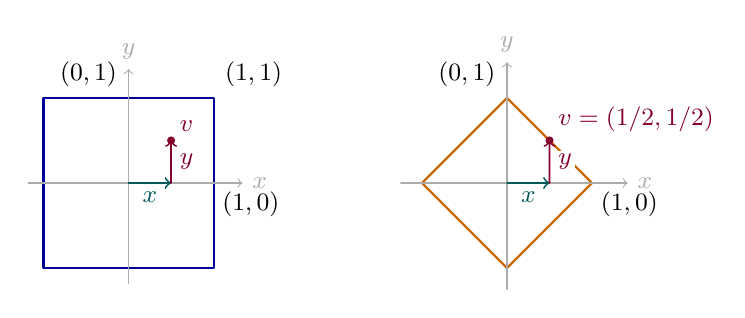
\begin{tikzpicture}[
  scale=1.08,
  font=\small,
  line cap=round,
  line join=round,
  axis/.style={gray!65, ->},
  maxball/.style={blue!60!black, thick},
  sumball/.style={orange!80!black, thick},
  xcomp/.style={teal!70!black, ->, line width=0.65pt},
  ycomp/.style={purple!70!black, ->, line width=0.65pt},
  pointlabel/.style={purple!70!black, fill=white, inner sep=1pt},
  metriclabel/.style={fill=white, inner sep=1pt}
]
  \begin{scope}
    \draw[maxball] (-1,-1) rectangle (1,1);
    \draw[axis] (-1.18,0) -- (1.34,0) node[right] {$x$};
    \draw[axis] (0,-1.18) -- (0,1.34) node[above] {$y$};
    \coordinate (vmax) at (0.5,0.5);
    \draw[xcomp] (0,0) -- (0.5,0);
    \draw[ycomp] (0.5,0) -- (vmax);
    \fill[purple!70!black] (vmax) circle (1.35pt);
    \node[pointlabel, above right=2pt] at (vmax) {$v$};
    \node[teal!70!black, below=2pt, metriclabel] at (0.25,0) {$x$};
    \node[purple!70!black, right=2pt, metriclabel] at (0.5,0.25) {$y$};
    \node[above left=3pt, metriclabel] at (0,1) {$(0,1)$};
    \node[above right=3pt, metriclabel] at (1,1) {$(1,1)$};
    \node[below right=2pt, metriclabel] at (1,0) {$(1,0)$};
  \end{scope}

  \begin{scope}[xshift=4.45cm]
    \draw[sumball] (0,1) -- (1,0) -- (0,-1) -- (-1,0) -- cycle;
    \draw[axis] (-1.25,0) -- (1.42,0) node[right] {$x$};
    \draw[axis] (0,-1.25) -- (0,1.42) node[above] {$y$};
    \coordinate (vsum) at (0.5,0.5);
    \draw[xcomp] (0,0) -- (0.5,0);
    \draw[ycomp] (0.5,0) -- (vsum);
    \fill[purple!70!black] (vsum) circle (1.35pt);
    \node[pointlabel, above right=2pt] at (vsum) {$v=(1/2,1/2)$};
    \node[teal!70!black, below=2pt, metriclabel] at (0.25,0) {$x$};
    \node[purple!70!black, right=2pt, metriclabel] at (0.5,0.25) {$y$};
    \node[above left=3pt, metriclabel] at (0,1) {$(0,1)$};
    \node[below right=2pt, metriclabel] at (1,0) {$(1,0)$};
  \end{scope}
\end{tikzpicture}

  \caption{The maximum-metric unit ball is square; the sum-metric unit ball is diamond-shaped.}
  \label{fig:product-metric-unit-balls}
\end{illustrationfigure}

\begin{proposition} \label{prop:product-metric-comparison} \hlt{Product Metrics and Comparisons}\\
Let $(X,d_X)$ and $(Y,d_Y)$ be metric spaces. The product distance functions $d_E,d_{\max},d_{\mathrm{sum}}$ satisfy:
\begin{enumerate}[label=(\roman*)]
\setlength{\itemsep}{0pt}
\item $d_E,d_{\max},d_{\mathrm{sum}}$ are metrics on $X\times Y$;
\item $d_{\max}\leq d_E\leq d_{\mathrm{sum}}\leq2d_{\max}$;
\item they are pairwise equivalent and have the same convergent sequences.
\end{enumerate}
\begin{proof}
\begin{enumerate}[label=(\roman*)]
\setlength{\itemsep}{0pt}
\item Let $p=(x,y)$, $p'=(x',y')$, and $p''=(x'',y'')$, and set $(a,b,c,e)\defeq(d_X(x,x'),d_Y(y,y'),d_X(x',x''),d_Y(y',y''))$.\\
All three functions are nonnegative and symmetric, and each vanishes iff $a=b=0$, equivalently $p=p'$.\\
By the component triangle inequalities, $d_{\mathrm{sum}}(p,p'')\leq a+b+c+e=d_{\mathrm{sum}}(p,p')+d_{\mathrm{sum}}(p',p'')$.\\
Likewise, $d_{\max}(p,p'')\leq\max\{a+c,b+e\}\leq\max\{a,b\}+\max\{c,e\}$ by the component triangle inequalities.\\
By Theorem \ref{thm:triangle-inequality-inner-product}(i), $d_E(p,p'')\leq\sqrt{(a+c)^2+(b+e)^2} \leq\sqrt{a^2+b^2}+\sqrt{c^2+e^2}$.
\item For $p=(x,y)$ and $p'=(x',y')$, set $a\defeq d_X(x,x')$ and $b\defeq d_Y(y,y')$. Then $\max\{a,b\}\leq\sqrt{a^2+b^2}\leq a+b\leq2\max\{a,b\}$.
\item The metrics are pairwise equivalent by (ii) and Definition \ref{def:equivalent-metrics}. Their convergent sequences coincide by Proposition \ref{prop:equivalent-metrics-preserve-tests}(iii).
\end{enumerate}
\hlt{Structural Commentary}: Component triangle inequalities prove the metric axioms; uniform comparison transfers convergence.\\
\hlt{Key Insight}: Maximum and sum bounds trap the Euclidean product distance.
\end{proof}
\end{proposition}

\begin{proposition} \label{prop:sequential-closure-criterion} \hlt{Sequential Closure Criterion}\\
Let $X$ be a metric space, let $E\subseteq X$, and let $p\in X$. Then $p\in\overline{E}\Longleftrightarrow(\exists u:\N\to E)\,u_n\to p$.
\begin{proof}
\begin{enumerate}[label=\roman*.]
\setlength{\itemsep}{0pt}
\item[$(\Rightarrow)$] Suppose $p\in\overline{E}$. By Definition \ref{def:adherent-points-and-closure}, $(\forall n\in\N)\,E\cap B_{\frac{1}{n}}(p)\neq\emptyset$. Choose $(p_n)$ with $(\forall n\in\N)\,p_n\in E\cap B_{\frac{1}{n}}(p)$.\\
Given $\varepsilon>0$, choose $N\in\N$, $N\varepsilon>1$ by Theorem \ref{thm:archimedean-and-rational-density}(i). Then $(\forall n\geq N)\,d(p_n,p)<\frac{1}{n}\leq\frac{1}{N}<\varepsilon$, so $p_n\to p$ by Definition \ref{def:sequence-convergence-metric}.
\item[$(\Leftarrow)$] Suppose $(\forall n\in\N)\,p_n\in E$ and $p_n\to p$. Given $r>0$, choose $N\in\N$ with $d(p_N,p)<r$.\\
Then $p_N\in E\cap B_r(p)$, so $p\in\overline{E}$ by Definition \ref{def:adherent-points-and-closure}.
\end{enumerate}
\hlt{Structural Commentary}: Adherence selects points from shrinking balls; convergence returns a witness to each ball.\\
\hlt{Key Insight}: The radii $n^{-1}$ encode all positive metric scales.
\end{proof}
\end{proposition}

\begin{theorem} \label{thm:closed-sets-and-limit-points-via-sequences} \hlt{Closed Sets and Limit Points via Sequences}\\
Let $X$ be a metric space and $E\subseteq X$.
\begin{enumerate}[label=(\roman*)]
\setlength{\itemsep}{0pt}
\item $(\forall p\in X)\,[p\in E^{\operatorname{acc}}\Longleftrightarrow(\exists u:\N\to E\setminus\{p\})\,u_n\to p]$.
\item $E$ is closed iff $(\forall p\in X)(\forall u:\N\to E)\,[u_n\to p\Longrightarrow p\in E]$.
\end{enumerate}
\begin{proof}
\begin{enumerate}[label=(\roman*)]
\setlength{\itemsep}{0pt}
\item[$(i)$] ($\Rightarrow$) Fix $p\in E^{\operatorname{acc}}$. A sequence $(p_n)$ in $E\setminus\{p\}$ with $p_n\to p$ exists by Theorem \ref{thm:metric-sequence-basic-properties}(iii).
\item[$(i)$] ($\Leftarrow$) Fix $p\in X$ and suppose $(\forall n\in\N)\,p_n\in E\setminus\{p\}$ with $p_n\to p$.\\
Given $r>0$, choose $N\in\N$ with $p_N\in B_r(p)$. Then $p_N\in B_r(p)\cap(E\setminus\{p\})$, so $p\in E^{\operatorname{acc}}$.
\item[$(ii)$] ($\Rightarrow$) Suppose $E$ closed, $(\forall n\in\N)\,p_n\in E$, $p_n\to p\in X$; $p\in\overline{E}$ by Proposition \ref{prop:sequential-closure-criterion}. Since $\overline{E}=E$ by Theorem \ref{thm:closure-smallest-closed-containing-set}(ii), $p\in E$.
\item[$(ii)$] ($\Leftarrow$) Assume the sequential limit condition, and fix $p\in\overline{E}$.\\
By Proposition \ref{prop:sequential-closure-criterion}, some sequence $(p_n)$ in $E$ converges to $p$, so $p\in E$ by the assumed condition.\\
Thus $\overline{E}\subseteq E$, while $E\subseteq\overline{E}$ by Definition \ref{def:metric-closure}. Therefore $E=\overline{E}$, and $E$ is closed by Theorem \ref{thm:closure-smallest-closed-containing-set}(ii).
\end{enumerate}
\hlt{Structural Commentary}: Punctured-ball sequences characterize accumulation; ordinary ball sequences characterize closure.\\
\hlt{Key Insight}: Closedness is exactly retention of limits of internal sequences.
\end{proof}
\end{theorem}

\begin{theorem} \label{thm:subsequential-limits-closed} \hlt{Subsequential Limits Form a Closed Set}\\
For a sequence $(p_n)$ in a metric space $X$, the set of all subsequential limits is closed.
\begin{proof}
\begin{enumerate}[label=(\roman*)]
\setlength{\itemsep}{0pt}
\item \hlt{Approximation}: Let $E^*$ be set of subsequential limits, $q\in(E^*)^{\operatorname{acc}}$. Choose $(x_i)$ with $(\forall i\in\N)\,x_i\in(E^*\setminus\{q\})\cap B_{\frac{1}{2i}}(q)$.
\item \hlt{Diagonal selection}: Each $x_i$ satisfies condition (i) by Proposition \ref{prop:sequence-limit-points-subsequential-limits}, direction $(ii)\Rightarrow(i)$.\\
Set $n_0\defeq0$ and recursively choose $n_i>n_{i-1}$ with $d(p_{n_i},x_i)<\frac{1}{2i}$ by condition (i).
\item \hlt{Closure}: By the triangle inequality, $(\forall i\in\N)\,d(p_{n_i},q)<\frac{1}{i}$. Given $\varepsilon>0$, choose $I\in\N$ with $I\varepsilon>1$ by Theorem \ref{thm:archimedean-and-rational-density}(i).\\
Then $(\forall i\geq I)\,d(p_{n_i},q)<\frac{1}{i}\leq\frac{1}{I}<\varepsilon$, so $p_{n_i}\to q$ by Definition \ref{def:sequence-convergence-metric}. Thus $q\in E^*$; $(E^*)^{\operatorname{acc}}\subseteq E^*$, $E^*$ closed by Definition \ref{def:metric-topology-core-definitions}.
\end{enumerate}
\hlt{Structural Commentary}: Shrinking approximants and increasing original indices combine into one diagonal subsequence.\\
\hlt{Key Insight}: Each diagonal term is simultaneously later and closer to $q$.
\end{proof}
\end{theorem}

\begin{proofmethod} \label{meth:metric-topology-proof-patterns} \hlt{Metric Proof Patterns}
\begin{enumerate}[label=(\roman*)]
\setlength{\itemsep}{0pt}
\item To prove openness of $G$, fix $x\in G$ and construct $r>0$ with $B_r(x)\subseteq G$; then $G$ is open by Definition \ref{def:metric-topology-core-definitions}.
\item To prove closedness of $F$, establish $F^{\operatorname{acc}}\subseteq F$ and conclude by Definition \ref{def:metric-topology-core-definitions}.\\
Alternatively, prove $F^c$ open and conclude by Corollary \ref{cor:closed-iff-complement-open}.
\item To identify $C=\overline{E}$, verify $E\subseteq C$, $C^{\operatorname{acc}}\subseteq C$, and $(\forall F\subseteq X)\,[(E\subseteq F\land F^{\operatorname{acc}}\subseteq F)\Longrightarrow C\subseteq F]$; $C=\overline{E}$ by Theorem \ref{thm:closure-smallest-closed-containing-set}.
\item For $\emptyset\ne E\subseteq X$, prove $\operatorname{dist}(p,E)=0$ and conclude $p\in\overline{E}$ by Proposition \ref{prop:set-distance-closure-criterion}.\\
Alternatively, construct $(p_n)$ in $E$ with $p_n\to p$ and conclude by Proposition \ref{prop:sequential-closure-criterion}.
\end{enumerate}
\end{proofmethod}
